\documentclass[12pt]{article}
\usepackage{sbc-template}
\usepackage{graphicx,xurl,placeins}
\graphicspath{{figures/lab02/}{paper/figures/lab02/}}
\usepackage[utf8]{inputenc}
\usepackage[T1]{fontenc}
\usepackage[brazil]{babel}
\usepackage{amsmath,amssymb,booktabs}
\usepackage[hidelinks]{hyperref}
\sloppy
\title{Além do Beta Tradicional: Assimetria, Heterogeneidade Setorial e Risco em Ações Brasileiras}
\author{Robson Dias Ferreira\inst{1}}
\address{Instituto de Informática -- Universidade Federal do Rio Grande do Sul (UFRGS)\\
Programa de Pós-Graduação em Computação (PPGC)\\
Disciplina CMP609 -- Introdução aos Métodos Computacionais em Finanças
\email{}}
\begin{document}
\maketitle
\begin{abstract}
We examine upside and downside market sensitivities in fixed samples of 80 Brazilian securities for 2016--2025 and 117 for 2021--2025, covering ten sectors. Daily log returns are paired with the B3 Ibovespa; overlapping securities are compared over a common period. Regime-specific regressions preserve classes, valid pairs and missingness. Although 59 of 80 decade contrasts indicate greater downside sensitivity, only two of 197 primary HAC/Holm tests reject symmetry, with opposite signs. A complementary Monte Carlo rank envelope retains one rejection within specified error mechanisms. Temporal non-rejections coexist with low power and do not establish stability or future persistence. Sector and historical-risk summaries reveal heterogeneous exposures. Rolling-origin next-return forecasts yield small, mixed incremental gains, and interval calibration exposes undercoverage. Retrospective selection, revised data and incomplete corporate-event verification restrict interpretation. The contribution is a reproducible conditional characterization with explicit inferential limits, without generalized asymmetry, predictive superiority or CAPM pricing claims.
\end{abstract}
\begin{resumo}
Examinamos sensibilidades de alta e baixa em amostras fixas de 80 ativos brasileiros em 2016--2025 e 117 em 2021--2025, em dez setores. Retornos logarítmicos diários são pareados ao Ibovespa B3; os ativos sobrepostos são comparados no período comum. Regressões com interceptos por regime preservam classes, pares válidos e ausências. Embora 59 dos 80 contrastes da década indiquem maior sensibilidade nas quedas, somente dois dos 197 testes principais HAC/Holm rejeitam simetria, com sinais opostos. Um envelope complementar de postos Monte Carlo conserva uma rejeição sob mecanismos de erro especificados. Não rejeições temporais coexistem com baixa potência e não demonstram estabilidade ou persistência futura. Resumos setoriais e de risco histórico mostram exposições heterogêneas. Previsões do retorno seguinte com origens móveis apresentam ganhos incrementais pequenos e mistos; sua calibração revela subcobertura dos intervalos. Seleção retrospectiva, dados revisados e auditoria econômica incompleta restringem a interpretação. A contribuição é uma caracterização condicional reproduzível com limites inferenciais explícitos, sem alegar assimetria generalizada, superioridade preditiva ou precificação CAPM.
\end{resumo}
\section{Introdução}
Uma inclinação única em relação ao mercado pode ocultar respostas
diferentes em altas e quedas. Essa possibilidade motiva estimar betas
condicionais, mas não estabelece, por si, sua estabilidade ou utilidade
prospectiva. O problema é determinar quanto a assimetria estimada depende de
liquidez, composição e janela, distinguindo associação transversal,
mudança temporal e identificação individual.

O CAPM relaciona retorno esperado e exposição ao mercado
\cite{sharpe1964}; a literatura de risco de queda oferece motivação
econômica para considerar estados adversos \cite{ang2006}.
Levi e Welch \cite{leviwelch2020} questionam a vantagem prospectiva
dos betas assimétricos. Nosso contraste descreve projeções de retornos
observados, sem testar prêmio de risco ou previsão do beta futuro.
Na versão de trabalho de Ang et al. \cite{ang2004working}, o evento
condicionante usa o excesso de retorno abaixo de sua média; aqui,
o limiar é zero no log-retorno observado do mercado.

No Brasil, Fortunato et al. \cite{fortunato2010} examinam medidas
de risco e custo de capital em 50 ações com dados mensais de 1995--2006.
Faria e Santos \cite{faria2010} comparam CAPM/D-CAPM em 21 ações,
de 2006--2010, com Ibovespa e Selic. Seu D-CAPM trunca excessos
positivos do ativo e do mercado; as projeções centralizadas por regime
adotadas aqui têm outro estimando. Estrada \cite{estrada2002,estrada2007}
também usa definições distintas. Frequência, referencial e universo
precisam ser harmonizados antes de comparar sinais ou magnitudes.
O suplemento amplia esse contexto, sem reivindicar pioneirismo brasileiro.

A liquidez oferece duas interpretações que precisam ser distinguidas.
Acharya e Pedersen \cite{acharyapedersen2005} modelam remuneração
associada a custos e covariâncias de liquidez; Brunnermeier e Pedersen
\cite{brunnermeierpedersen2009} relacionam negociação e financiamento,
com espirais sob condições específicas. Chordia et al.
\cite{chordia2000} documentam componentes comuns de liquidez.
Esses mecanismos econômicos coexistem com negociação infrequente e
assincronia na mensuração. Volume financeiro é uma aproximação de atividade,
não uma medida direta de spread, custo ou risco de liquidez; nossa
regressão não testa os modelos de precificação dessas referências.


Investigamos 80 ativos em 2016--2025 e 117 em 2021--2025, em dez setores.
O recorte dos mesmos 80 no período recente permite distinguir,
descritivamente, janela e composição. O núcleo é a existência e a
sensibilidade temporal da assimetria; setores e risco organizam a
heterogeneidade. Indicadores técnicos e métodos sequenciais de
covariância permanecem extensões não executadas. A contribuição empírica é quantificar a sensibilidade da assimetria a
universo, liquidez e controles observados, articulando evidência agregada,
identificação individual e limites da inferência. A associação condicional
é exploratória e não foi pré-registrada; resultados anteriores eram conhecidos.

\section{Dados, perguntas e alcance}
\subsection{Amostras e construção dos retornos}
As amostras são fixas: 80 ativos em 2016--2025 e 117 em 2021--2025.
A primeira está contida na segunda; não há seleção anual, colapso
de classes, agregação por emissor ou pesos empresariais. Os grupos
correspondem a 76 e 112 emissores. Classes distintas podem ser dependentes.
A seleção considera volume financeiro negociado em 2025 e presença
histórica, produzindo vieses retrospectivo e de sobrevivência.
O cadastro setorial datado não reconstrói classificações disponíveis
em cada época \cite{b3setorial}.

Ativo e Ibovespa são pareados no calendário B3. Usam-se log-retornos
diários, construídos de um cache consultado por yfinance e confrontado
com fontes B3 \cite{yfinance,b3cotacoes,b3layout,b3empresas}.
Preços são insumos da construção e auditoria; as regressões utilizam
retornos. A referência observada contém reconciliações rastreadas,
sem pressupor harmonização econômica e tributária integral entre
fatores do fornecedor e o índice de retorno total \cite{b3indices}.

Cinco retornos diários permanecem não identificáveis: ABCB4 em 4 e 5/1/2016
e UGPA3 em 28--30/6/2021. Preservam-se ausências, sem interpolação
ou distribuição de pontes acumuladas entre dias. Duas ausências de
ANIM3 em 20 e 23/11/2020 elevam a sete o total da década; quatro
de AZUL4 e três de UGPA3 também totalizam sete no recente.
Nos 80 comuns há três. Light em 30/10/2024 foi reconciliada
\cite{abcb2015,ultra2021,light2024,b3lightcustodia,b3lightnegocios,b3diaria2026}.
As mesmas matrizes e máscaras são reutilizadas nas novas análises.

Embora 73 dos 74 ativos de uma frente documental tenham revisão local,
nenhum dos 197 históricos ativo--período cumpre todos os requisitos
de homologação econômica. Isso significa certificação incompleta,
não erro em todos os retornos. Identidade, quantidade, bordas, ANIM3
e harmonização de caixa continuam entre as pendências. A tabela oficial
Frasle foi extraída, mas contém inconsistências cronológicas preservadas
\cite{frasinventario2026}. Registros e documentos estão no material suplementar.

\subsection{Hipóteses e estimandos}
Sejam $r_{it}$ e $m_t $ os log-retornos do ativo e do mercado.
Define-se $\Delta_i=\beta_i^+-\beta_i^-$, com regimes $m_t>0$ e $m_t<0$.
A H1 de pesquisa é existir diferença entre exposições em parte dos ativos;
os testes individuais são bilaterais, $H_{0i}:\Delta_i=0$.
$\Delta_i<0$ indica maior inclinação estimada nas quedas, sem impor
uma alternativa unilateral. Contar sinais negativos não testa prevalência.

A H2 é que a assimetria pode mudar entre quinquênios. Para os mesmos 80,
\begin{equation}
\theta_i=\Delta_{i, 2021-2025}-\Delta_{i, 2016-2020}.
\end{equation}
Testar cada $\theta_i $ e testar média ou mediana do conjunto são perguntas
distintas. A mediana das diferenças pareadas não é a diferença de medianas.
Não foi definida margem de equivalência econômica; não rejeição não
estabelece simetria, constância ou persistência futura.

As hipóteses foram explicitadas com resultados anteriores conhecidos.
As análises complementares são exploratórias, não pré-registradas;
protocolos antecedem seus próprios resultados, não o conhecimento das
análises anteriores. A pergunta condicional adicional é se a associação
entre liquidez de 2015 e $\Delta$ inicial permanece ao controlar porte,
setor e exposição tradicional. A Tabela~\ref{tab:familias} distingue as
famílias; não se alega controle de erro sobre todo o programa.

\begin{table}[htbp]\centering\footnotesize
\caption{Alvos e multiplicidade. Ajustes separados por bloco, salvo HAC.
ICs bootstrap são marginais nominais, não intervalos simultâneos.}
\label{tab:familias}\begin{tabular}{p{.16\textwidth}p{.58\textwidth}p{.16\textwidth}}
\toprule
Família & Hipóteses/alvos & Ajuste\\\midrule
Individual & $\Delta_i=0$ em 80 longos e 117 recentes & Holm197\\
Temporal & Mudança em 80; sinais anuais em 80/117 & Holm474\\
Níveis & Média/mediana de três painéis e duas exclusões & Holm10\\
Metades & Média/mediana inicial e mudança pareada & Holm4\\
Crise & Média/mediana da mudança em duas exclusões & Holm4\\
Microestrutura & Dois resumos, três modelos, três painéis & Holm18\\
Seleção 2015 & Inicial/mudança; níveis da década e recente, por universo/variante & Holm4/2\\
Postos iniciais & Dois alvos, duas coortes, duas máscaras & Holm8\\
Controles & Coeficiente de log-volume: oito modelos, duas coortes & Holm16\\
Mudanças & Nível/mudança da liquidez vs. $\theta$, duas coortes & Holm4\\
Continuidades & Média inicial/postos, duas coortes & Holm4\\\bottomrule
\end{tabular}

\end{table}

\section{Métodos}
\subsection{Estimação e incerteza}
Com pares válidos por ativo e janela, estimam-se
\begin{align}
\widehat\beta_i&=\widehat{\mathrm{Cov}}(r_i,m)/\widehat{\mathrm{Var}}(m),\\
\widehat\beta_i^{s}&=\frac{\widehat{\mathrm{Cov}}(r_i,m\mid sm>0)}{\widehat{\mathrm{Var}}(m\mid sm>0)},\quad s\in\{-1,+1\},\qquad
\widehat\Delta_i=\widehat\beta_i^+-\widehat\beta_i^-.
\end{align}
Cada regime tem centralização própria. Dias neutros entram no beta
tradicional e no risco, mas não no contraste condicional. A regressão
conjunta equivalente, nos dias não neutros, é
\begin{equation}
r_{it}=a_i+g_iD_t+b_im_t+\Delta_iD_tm_t+e_{it},
\quad D_t=\mathbf{1}\{m_t>0\}.
\end{equation}
Assim, $b_i=\beta_i^-$ e $g_i $ permite interceptos próprios;
não representa uma descontinuidade causal. A covariância conjunta
preserva a dependência entre as duas inclinações.

Exigem-se 200 pares, 60 por regime, 95\% de cobertura elegível e variância
do mercado acima de $10^{-12}$. São salvaguardas contra ajustes curtos
e perdas de calendário, sem garantia de potência ou validade assintótica.
Não se relaxam pisos, preenchem lacunas ou descartam insuficiências.
A referência individual usa HAC/Bartlett5, correção $n/(n-k)$ e
aproximação normal \cite{neweywest1987}. Escores ficam na grade original;
ausências não comprimem o calendário. Holm a 5\% ajusta 197 posições
\cite{holm1979}; os 80 comuns reutilizam as decisões dos 117.
O suplemento detalha os 474 testes temporais, potência e complemento
Monte Carlo, cuja proteção é restrita às leis declaradas
\cite{morris2019,dufour2006,phipson2010}.

Para o universo fixo $S $, $\mu_{\Delta,S}=N^{-1}\sum_{i\in S}\Delta_i $
e $q_{\Delta,S}=\mathrm{mediana}_{i\in S}\Delta_i $ são resumos dos ativos,
sem construir uma carteira. O bootstrap usa 4.999 reamostragens móveis
não circulares de sessões \cite{kunsch1989}, reestimando as inclinações.
Mercado, ativos e ausências compartilham os índices. Sorteiam-se
separadamente 2016--2020 e 2021--2025, mantendo durações; 80 comuns
e 117 recentes compartilham exatamente os sorteios recentes.

O bloco principal é 21 sessões; 5 e 63 são sensibilidades reportadas.
Com $T^*$ reestimado, usam-se
\begin{equation}
p=\frac{1+\#\{|T^*-\widehat T|\ge|\widehat T|\}}{5000}
\end{equation}
e ICs básicos marginais nominais de 95\%. A centralização é aproximada;
o acréscimo de um não produz teste Monte Carlo exato. Valores-p bilaterais
centrados e ICs básicos assimétricos não são duais. A calibração
abaixo mede seu desempenho separadamente; cruzar zero no gráfico
não substitui o teste ajustado. A interpretação dos blocos requer
regularidade e dependência suficientemente fraca nos trechos.

As famílias agregadas e suas proteções constam da Tabela~\ref{tab:familias}.
Holm 30 permanece sensibilidade conservadora sobre F10 nos três blocos.

\subsection{Sensibilidade da mudança à crise}
\label{sec:crise}
Para cada exclusão $q $, define-se
$\theta_{i,q}=\Delta_{i, 2021-2025}-\Delta_{i, 2016-2020\setminus q}$.
Retiram-se março/2020 ou 2020-S1 apenas da primeira metade; a segunda
e os 80 ativos são mantidos. O contraste é calculado por ativo antes
de resumir. Cada trecho contíguo restante é reamostrado separadamente,
sem blocos atravessando a lacuna. Reutilizam-se os bancos originais
das exclusões e o mesmo banco recente, reproduzindo também o G original.

A nova família H4 reúne média/mediana de $\theta $ nas duas exclusões,
com Holm 4 por bloco. Ela tem composição diferente de G4: a tabela
informa valores brutos e ajustados de ambas, sem comparar suas decisões
como se diferissem apenas nos dados. Nenhum sorteio inválido é substituído;
a inferência do alvo seria retida. Os ICs das novas máscaras não
receberam validação própria de cobertura. Excluir períodos muda o alvo
e a precisão, sem identificar uma causa ou uma quebra estrutural única.

\subsection{Calibração e diagnóstico dos mecanismos}
\label{sec:calibracao}
A calibração preservada usa 1.000 réplicas em seis mecanismos, com os
mesmos 4.999 sorteios internos/bloco 21. Mantém mercado, máscaras,
escalas individuais estimadas e dependência por fator comum de variância 0,3.
Inclui normal iid, componentes t5 heterocedásticos, t5/AR0,3 e estresses
GARCH t5, quebra de escala e AR 0,6. As famílias F10/G4 são avaliadas
separadamente sob nulidade global individual; isso não demonstra controle
forte para toda configuração de efeitos, nula agregada ou lei financeira.
H4, modelos dinâmicos/semanais e outros blocos não foram calibrados.
O gerador condiciona no caminho observado do mercado e da escala;
o bootstrap de pares também reamostra o desenho e não studentiza
$T^*-\widehat T$. Isso pode alterar a concentração dos pesos em
sessões de alta variância. É uma explicação plausível para a diferença
de precisão, não uma decomposição demonstrada da subcobertura.


A escala heterocedástica é proporcional a
$\sqrt{0,5+0,5m_{t-1}^2/\overline{m^2}}$, normalizada para
$T^{-1}\sum h_t^2=1$. Isso não iguala a precisão dos estimadores:
variância colocada onde o contraste tem maior peso produz outro efeito.
Se $a_{ti}=\sigma_iw_{it}/N $ e $w_{it}$ calcula $\widehat\Delta_i $,
na ausência de AR a variância condicional da média é
\begin{equation}
\sum_t h_t^2\left[0,3\left(\sum_i a_{ti}\right)^2+
0,7\sum_i a_{ti}^2\right].
\end{equation}
A fórmula AR completa e sua conferência independente estão no suplemento.
O estresse de quebra multiplica dois fatores normalizados; o produto
tem média quadrática 1,02955. Nenhum gerador foi alterado após os resultados.

Como diagnóstico exploratório, transformam-se os valores-p observados
pela CDF empírica dos valores-p nulos de cada mecanismo:
$\widetilde p_{jg}=(1+\#\{p^0_{jgr}\le p_j\})/1001$.
Recalibram-se todas as dez ou quatro marginais antes de reordenar Holm.
O banco existente não fornece validação independente dessa transformação;
contagens, incerteza Monte Carlo e alcance condicionado aos parâmetros
estimados são reportados. Esses diagnósticos não substituem os testes
originais, corrigem seus ICs ou ampliam a garantia do complemento individual.

\subsection{Setores, risco e especificações alternativas}
Por setor, apresentam-se mediana/IQR e agrupamento pontual $\eta^2$;
erro de estimação e composição impedem lê-lo como efeito causal ou
fração do risco explicada. Risco é descrito por volatilidade diária,
$R^2$ do modelo de mercado e ES95 da perda simples $L=1-\exp(r)$,
com massa fracionária na fronteira \cite{rockafellar1999}. São medidas
históricas, sem previsão ou ICs próprios.

A sensibilidade à assincronia adapta somas de coeficientes de Dimson
\cite{dimson1979}, com uma defasagem ou um avanço/defasagem e regime
definido pelo mercado contemporâneo. São outros estimandos descritivos;
avanços são usados apenas no ajuste retrospectivo. Retornos semanais
somam logs de semanas completas; uma ausência diária torna a semana
do ativo ausente. A família micro 18 reúne dois resumos, três modelos
e três painéis; os blocos correspondem a 21/5/63 sessões ou 4/1/13 semanas.
Seu tamanho não foi calibrado. Fórmulas, resultados completos e demais
sensibilidades permanecem no suplemento e nos exports.


\subsection{Seleção anterior ao período e liquidez}
Uma análise secundária reconstrói as cotações oficiais de 2015--2025,
por ISIN, a partir de onze ZIPs B3 autenticados já existentes.
Comparam-se os 80 originais com 80 escolhidos uma única vez pelo volume
financeiro médio por sessão em 2015, exigindo presença em pelo menos
90\% dos pregões daquele ano. Não se alteram os universos principais.
A elegibilidade posterior é reportada separadamente por alvo; selecionar
antes do período não elimina a seleção decorrente de perdas de identidade
ou de cobertura. Mantêm-se somente pares de pregões consecutivos,
sem distribuir retornos acumulados. Dividendos não são harmonizados;
uma regra de extremos/fatores gera 83 marcações de eventos, ainda
sem validação econômica integral. A reconstrução literal é um diagnóstico;
a variante usada para interpretação preserva adicionalmente as sete
ausências documentadas dos 80, incluindo os cinco dias de direitos.
Não se substitui a referência auditada por essa máscara heurística.

A associação de postos entre liquidez inicial e $\Delta$ inicial usa
4.999 sorteios síncronos, reestimando os betas, com coortes fixas e
sem reamostrar ativos como unidades iid. As associações anteriores
com $\theta$ são preservadas no suplemento, com seu Holm 8 original;
não constituem confirmação independente, pois $\theta$ já contém
$-\Delta_{2016-2020}$. Acoplamento e regressão à média são explicações
possíveis, sem implicar uma correlação negativa necessária.

Na análise condicional adicional, ajusta-se por ativo
\begin{equation}
 \widehat\Delta_{i, 2016-2020}=a+\lambda\log V_{i, 2015}
 +\gamma\log C_{i, 2015}^{\mathrm{div}}
 +\sum_s\zeta_s\mathbf1\{S_i=s\}+\eta\widehat\beta_{i, 2016-2020}+u_i.
\end{equation}
$V$ é volume financeiro médio por sessão. $C^{\mathrm{div}}$ combina
quantidades emitidas ou integralizadas, divulgadas até 31/12/2015,
e preços de fechamento por classe em 30/12/2015 \cite{cvmfre}.
É aproximação de capitalização divulgada, sem certificar quantidade
exata no fim do ano, ações em tesouraria ou free float. Classes sem
preço inequívoco e controles ausentes não são imputados. As versões
arquivadas e o cadastro setorial introduzem limitações de vintage.
Oito subconjuntos dos três controles usam os mesmos casos completos
em cada coorte. Exigem-se 40 ativos, 10 graus de liberdade residuais
e posto completo: salvaguardas de estabilidade, não garantia de potência.
Os modelos completos têm nove setores representados; as amostras
principais continuam nos dez setores originais.

Em cada sorteio, reestimam-se conjuntamente $\Delta$, beta tradicional
e a regressão transversal; porte, setor e volume de 2015 ficam fixos.
Holm 16 cobre oito modelos em duas coortes por bloco. Estimam-se também
$\rho_S(\theta,\log\bar V_{2021-2025}-\log\bar V_{2016-2020})$ e a
associação com o nível inicial, reestimando ambos os argumentos
variáveis nos mesmos sorteios; Holm 4 cobre dois alvos em duas coortes.
Volumes médios usam todos os pregões, com zero quando não há negócio
regular; isso não preenche retornos. ICs básicos e testes centrados
mantêm caráter aproximado e não foram calibrados para esses alvos.

\section{Resultados}
\subsection{Níveis, ativos e comparação comum}
A média de $\Delta $ na década é $-0,130668$, com $p_{Holm10}=0,0234$
no bloco 21; nos blocos 5/63,0,0080/0,0108. A mediana é $-0,135720$,
com $p_{Holm10}=0,0592$. Os painéis recentes têm resumos próximos
de zero e valores agregados ajustados 1 (Tabela~\ref{tab:niveis}).
Isso mantém os níveis recentes inconclusivos, sem evidência de equivalência.
Holm 30 produz 0,0624 para a média integral no bloco 21, uma sensibilidade
ao alcance da proteção entre escolhas. A Figura~\ref{fig:agregado}
apresenta os ICs nominais, sujeitos à calibração descrita adiante.

\begin{table}[htbp]\centering\small
\caption{Universos fixos. $p_m^*/p_q^*$: Holm 10, média/mediana, bloco 21.
Rej.$_i $: número de rejeições HAC5/Holm 197; 80 comuns reutilizam os 117.}
\label{tab:niveis}\begin{tabular}{lrrrrrrr}
\toprule
Recorte & $N$ & Média$\Delta$ & Mediana & $\Delta<0$ & $p^*_{m}$ & $p^*_{q}$ & Rej.$_i$\\
\midrule
2016--2025 & 80 & -0,1307 & -0,1357 & 59 & 0,0234 & 0,0592 & 2\\
80 comuns, 2021--2025 & 80 & -0,0101 & -0,0171 & 46 & 1,0000 & 1,0000 & 0\\
117, 2021--2025 & 117 & -0,0114 & -0,0082 & 62 & 1,0000 & 1,0000 & 0\\
\bottomrule
\end{tabular}

\end{table}
\begin{figure}[htbp]\centering
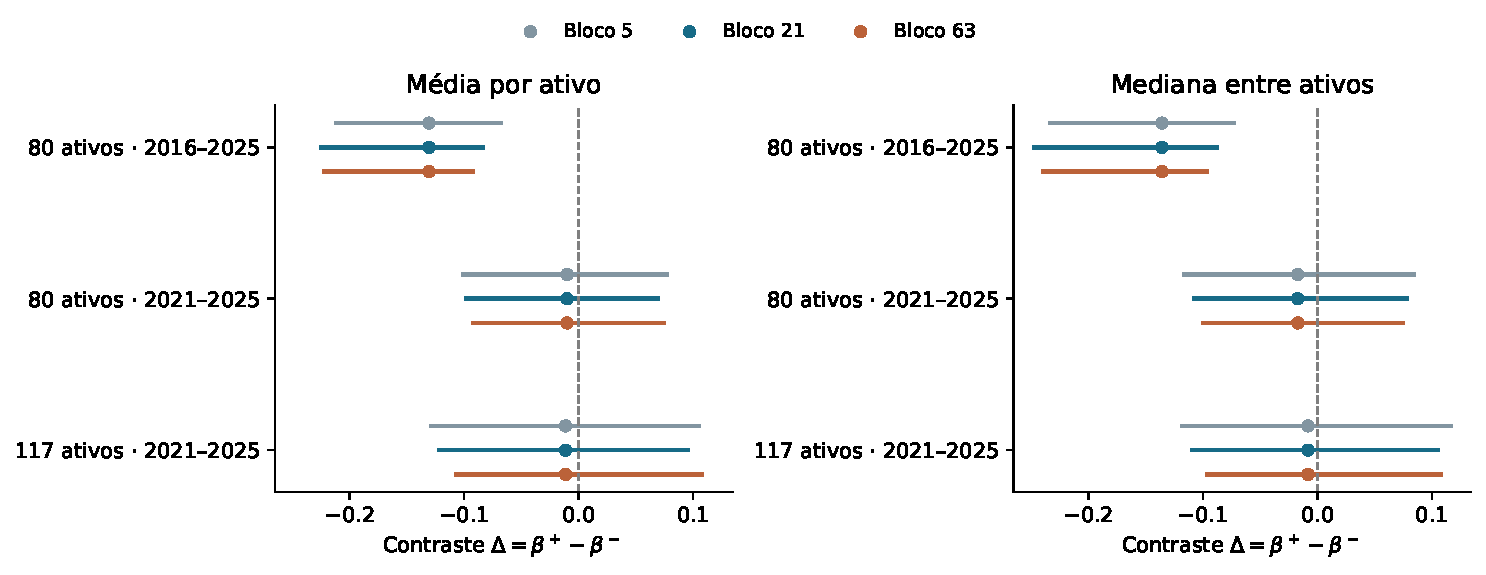
\includegraphics[width=\textwidth]{lab03f_agregado.pdf}
\caption{Níveis agregados e ICs básicos marginais nominais nos três blocos.
A cobertura não é uniformemente 95\%; cruzar zero não substitui Holm 10.}
\label{fig:agregado}
\end{figure}

Na família individual, VULC3 $(-0,496642;p_{Holm197}=0,002116)$
e BBDC4 $(0,246606;0,019561)$ rejeitam simetria, com sinais opostos;
nenhum recente rejeita. O complemento restrito às leis declaradas
mantém apenas VULC3 $(p=0,01970)$, enquanto BBDC4 passa a 0,09408.
As duas rejeições originais não sobrevivem às exclusões de crise
nas sensibilidades individuais. Identificação frágil e assimetria média
são achados distintos; 59 sinais negativos na década não testam prevalência.

\subsection{Mudança entre quinquênios e exclusões de 2020}
A média inicial é $-0,176760$, contra $-0,010080$ nos mesmos 80 recentes.
A mudança média pareada é $0,166680$, com $p_{Holm4}=0,0252$ em G4;
nos blocos 5/63,0,0224/0,0216. A mediana de $\theta $ é $0,135591$,
com 0,0508 no bloco 21 e 0,0594/0,0396 nos outros. A mediana é sensível
ao bloco; escolher 63 após observar a rejeição alteraria a interpretação.

As exclusões reduzem a mudança média para $0,125359$ sem março
e $0,145623$ sem 2020-S1. Os sinais permanecem positivos, mas nenhum
dos quatro alvos H4 rejeita na escolha principal: valores ajustados
de 0,1794 e 0,0680 para as médias (Tabela~\ref{tab:crise}).
A retirada apenas de março também leva o valor bruto da média a 0,0602;
sem o semestre, o bruto é 0,0170. Portanto, os dados preservam uma
diferença direcional e não estabelecem detecção ajustada uniforme.
Os ajustes usam famílias diferentes, explicitadas nos métodos.

\begin{table}[htbp]\centering\small
\caption{Mudança pareada dos 80. $p_{21}$: bruto; $p^*$: ajustado no bloco
indicado. Integral usa G4; exclusões usam a nova H4. São famílias distintas.}
\label{tab:crise}\begin{tabular}{llrrrrr}
\toprule
Primeira metade & Resumo & $\widehat\theta$ & $p_{21}$ & $p^*_{21}$ & $p^*_{5}$ & $p^*_{63}$\\
\midrule
Integral & Média & 0,1667 & 0,0126 & 0,0252 & 0,0224 & 0,0216\\
Integral & Mediana & 0,1356 & 0,0508 & 0,0508 & 0,0594 & 0,0396\\
Sem março/2020 & Média & 0,1254 & 0,0602 & 0,1794 & 0,1194 & 0,1386\\
Sem março/2020 & Mediana & 0,1029 & 0,1840 & 0,1840 & 0,1704 & 0,1498\\
Sem 2020-S1 & Média & 0,1456 & 0,0170 & 0,0680 & 0,0608 & 0,0448\\
Sem 2020-S1 & Mediana & 0,1447 & 0,0598 & 0,1794 & 0,1276 & 0,1386\\
\bottomrule
\end{tabular}

\end{table}
\begin{figure}[htbp]\centering
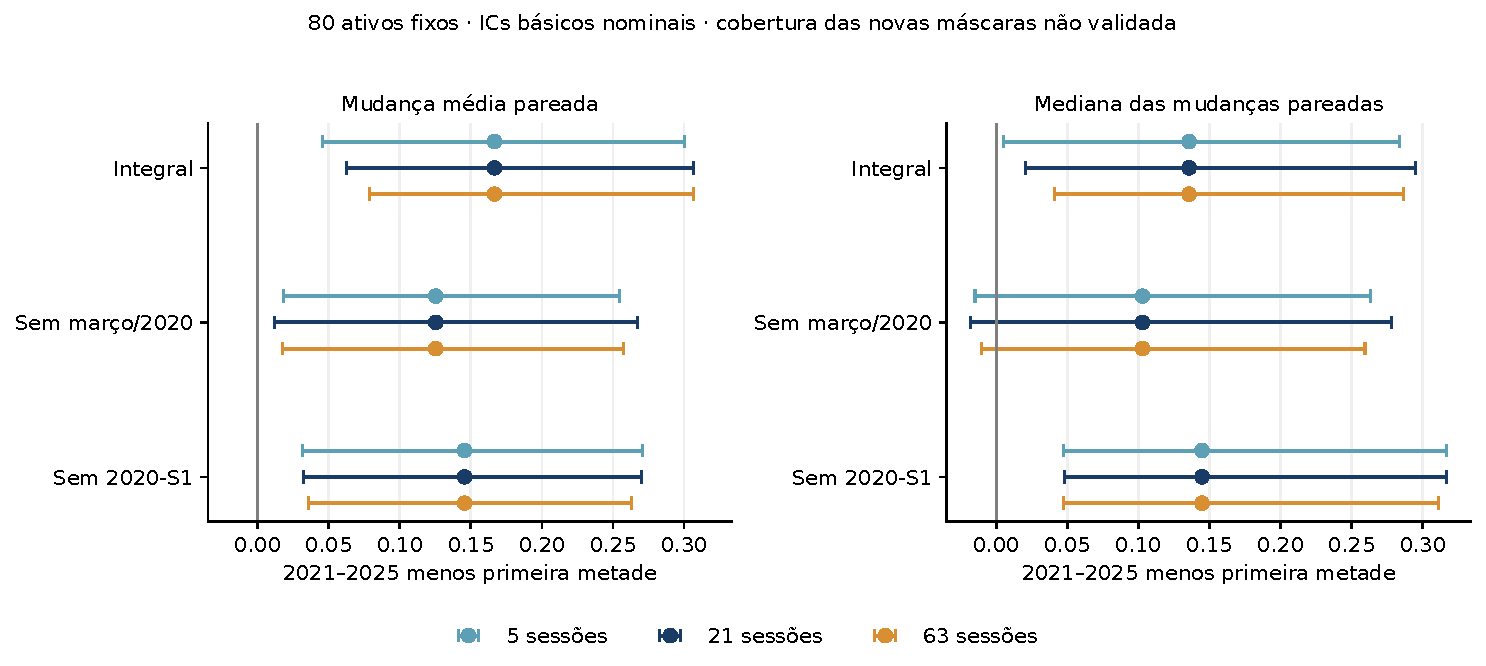
\includegraphics[width=\textwidth]{lab03h_crise.pdf}
\caption{Mudança pareada e ICs básicos nominais. Cobertura das máscaras novas
não validada; decisões usam os valores-p e famílias da Tabela~\ref{tab:crise}.}
\label{fig:crise}
\end{figure}

Sem 2020-S1, a média rejeita em 63 sessões $(p_{Holm4}=0,0448)$,
mas não em 5 ou 21. Essa sensibilidade é preservada. Reduzir o conjunto
de datas muda distribuição do mercado, ponderação temporal e precisão;
nem a rejeição nem sua ausência identifica o papel causal de março.
Nenhum teste temporal individual rejeita após as 474 posições originais;
esse alvo não contradiz um resultado agregado e tem outra potência.

\subsection{Calibração e escala dos mecanismos}
A cobertura da média da década é 94,8\% sob normalidade iid e 95,1\%
sob GARCH, com rejeição bruta 4,3/3,9\%. Nos outros mecanismos,
a cobertura desse mesmo alvo varia de 66,1 a 77,4\% (Tabela~\ref{tab:escala}).
Entre todos os 84 alvos/mecanismos, varia de 51,8 a 95,8\%; o mínimo
refere-se à média inicial sob AR 0,6, não a todos os ICs ou ao gerador normal.
As falhas são específicas de mecanismos e alvos, mas materiais.

\begin{table}[htbp]\centering\small
\caption{Nulidade global, mil réplicas por mecanismo. DP: dispersão da média
da década; EP: média dos erros-padrão bootstrap. Cob.: cobertura nominal 95\%.
São diagnósticos condicionais, sem critério de seleção de mecanismos.}
\label{tab:escala}\begin{tabular}{lrrrrr}
\toprule
Mecanismo & DP$\bar\Delta$ & EP$_{boot}$ & Cob.$\bar\Delta$(\%) & Cob.$\bar\theta$(\%) & DP/EP\\
\midrule
Normal iid & 0,044 & 0,046 & 94,8 & 94,2 & 0,96\\
t5 heteroc. & 0,139 & 0,094 & 77,4 & 79,8 & 1,48\\
t5 AR0,3 & 0,181 & 0,113 & 71,6 & 74,4 & 1,59\\
GARCH t5 & 0,044 & 0,045 & 95,1 & 94,6 & 0,98\\
Quebra t5 & 0,204 & 0,129 & 72,3 & 76,6 & 1,58\\
t5 AR0,6 & 0,220 & 0,134 & 66,1 & 67,1 & 1,64\\
\bottomrule
\end{tabular}

\end{table}

O EP bootstrap observado da média é 0,03725. Os DPs simulados variam
de 0,044 a 0,220, e o EP médio subestima essa dispersão em parte dos
mecanismos. Comparar essas escalas é informativo, mas o EP observado
não é uma dispersão verdadeira conhecida nem basta para definir realismo.
A fórmula condicional prevê DP de 0,14061 no mecanismo heterocedástico,
próximo de 0,13864 simulado. A dispersão elevada é compatível com o
posicionamento da variância em relação aos pesos do estimador, apesar
da normalização global. Não se elimina um estresse por ser desfavorável.

As FWERs ajustadas sob nulidade global são 1,6--3,1\% em F10 e 1,8--5,6\%
em G4. Sob AR 0,6, G4 alcança 5,6\%, Wilson 95\%[4,34; 7,20].
Não se demonstra controle forte ou validade geral. No diagnóstico CDF,
seguido de Holm na família completa, a média da década tem valores
de 0,01998 a 0,08092; sob AR0,3 e quebra, 0,08092/0,05395.
A mudança média varia de 0,02997 a 0,06194; a mediana, 0,05295--0,11988.
Esses números qualificam a leitura, sem validar um método substituto.
Banco finito, parâmetros estimados e nulas globais restringem seu alcance;
contagens e incerteza Monte Carlo estão no suplemento.

\subsection{Especificações alternativas, setores e risco}
Na década, as médias defasadas e semanal permanecem negativas.
Os valores brutos são pequenos em parte dos desenhos, mas nenhum
dos 18 alvos rejeita na escolha principal (tabela completa no suplemento).
Doze posições pertencem aos painéis recentes e seis à década;
a proteção cobre todas as afirmações declaradas. Isso não autoriza
reduzir a família após observar resultados. Semanalmente há cerca de 520
pares na década e 259 no recente, com intervalos mais largos.
No bloco 63, apenas a versão defasada da década rejeita média/mediana
com 0,0216/0,0238; o resultado não é uniforme entre escolhas.



A Figura~\ref{fig:periodo} conserva todos os dez anos, sem seleção anual.
As faixas são dispersão entre ativos, não ICs ou evidência de persistência.
Setores, trajetórias móveis, volatilidade, ES95 e a figura anual completa
de risco permanecem no suplemento. Não se identifica efeito causal de setor.
\begin{figure}[htbp]\centering
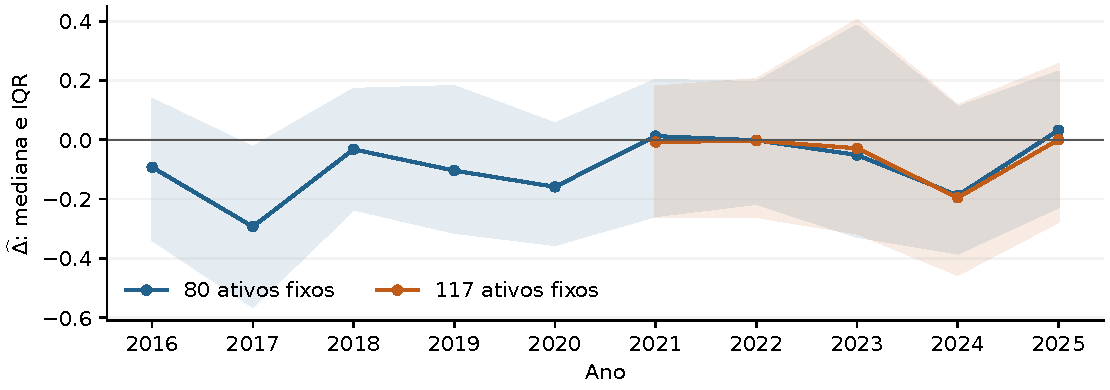
\includegraphics[width=\textwidth]{lab03j_assimetria_anual.pdf}
\caption{Período integral: mediana e IQR de $\widehat\Delta$ anual por ativo.
Amostras fixas; faixas descritivas sem interpretação de IC.}
\label{fig:periodo}
\end{figure}

Para explicitar a escala do coeficiente, um movimento simples de $-5\%$
corresponde a $m=\log(0,95)$. Na primeira metade integral,
a diferença média $(\beta^-_i-\beta^+_i)m $ é aproximadamente $-0,00907$,
ou $-0,91$ ponto percentual em escala logarítmica. É uma comparação
algébrica de componentes lineares, com um regime extrapolado ao mesmo $m $.
Interceptos e resíduos também integram retornos; isso não é perda esperada
de carteira, prêmio de risco ou equivalência econômica. Componentes
por ativo e por exclusão são exportados, sem pesos empresariais.


\subsection{Universo de 2015 e associação com liquidez}
A reconstrução independente reproduz os 48 resultados agregados externos
e as 83 marcações. A variante que preserva as lacunas dá resultados
próximos, apresentados na Tabela~\ref{tab:selecao}.
Na fonte COTAHIST, a média inicial é $-0,1685$ nos 78 originais elegíveis
e $-0,0857$ nos 64 elegíveis da seleção de 2015. A mudança média é
$0,1481$ em 77 pares originais e $0,0640$ em 46 pares do outro universo;
os valores ajustados são 0,0392 e 0,2576. São famílias secundárias
diferentes de F10: sua significância não pode ser comparada diretamente
à do resumo integral original. Entre os dois universos da tabela,
fonte e máscara são comuns; variam composição, elegibilidade e precisão.
A comparação com a referência original acrescenta diferenças de fonte
e ajustes. As diferenças pontuais não quantificam isoladamente viés
causal de seleção nem constituem um teste direto entre universos.

\begin{table}[!htbp]\centering\small
\caption{COTAHIST com lacunas preservadas, bloco 21. $p^*$: Holm 4 para
nível inicial/mudança e Holm 2 para década; não é a família F10 original.
A máscara de eventos permanece heurística.}
\label{tab:selecao}\begin{tabular}{llrrrr}
\toprule
Universo & Alvo & $N$ & Estimativa & $p$ & $p^*$\\
\midrule
Originais & Média$\Delta_{16-20}$ & 78 & -0,1685 & 0,0022 & 0,0088\\
Originais & Média$\theta$ & 77 & 0,1481 & 0,0196 & 0,0392\\
Originais & Média$\Delta_{16-25}$ & 78 & -0,1272 & 0,0010 & 0,0020\\
Seleção 2015 & Média$\Delta_{16-20}$ & 64 & -0,0857 & 0,0076 & 0,0304\\
Seleção 2015 & Média$\theta$ & 46 & 0,0640 & 0,1288 & 0,2576\\
Seleção 2015 & Média$\Delta_{16-25}$ & 48 & -0,0559 & 0,0166 & 0,0332\\
\bottomrule
\end{tabular}

\end{table}

Os universos compartilham 42 ISINs, dos quais 41 são elegíveis ao
contraste pareado. Só cinco pares vêm dos 38 ISINs exclusivos da
seleção de 2015; os originais exclusivos fornecem 36. Assim, o painel
pareado alternativo também está condicionado à permanência de identidade
e cobertura. Não rejeitar sua mudança não demonstra equivalência ou
uma população sem mudança. Uma sensibilidade separada encadeia apenas três mudanças documentadas
de código, sem alterar a unidade das análises principais: KROT3/COGN3,
ESTC3/YDUQ3 e TBLE3/EGIE3 \cite{cogna2019,yduqs2019,engie2016}.
Na seleção de 2015, os elegíveis iniciais passam de 64 a 67 e a média
fica em $-0,0894$; não se conclui o inventário de todas as sucessões.

Na união elegível, a associação inicial é positiva
($\rho_S=0,4928$, $N=100$, Holm 8=0,0168; Figura~\ref{fig:liquidez}).
O deslocamento bootstrap é $-0,1054$: compatível com ruído adicional
na ordenação, sem teorema geral de atenuação de Spearman sob erros
heterocedásticos e dependentes. A associação simples não controla porte
ou setor. Nos 62/76 casos completos, o coeficiente de log-volume cai
de 0,0647/0,0606 sem controles a 0,0316/0,0172 com todos os controles
(Tabela~\ref{tab:controles}). Os respectivos valores brutos são
0,0404/0,1462, e Holm 16 produz 0,2424/0,4386. Portanto, não há detecção
ajustada nos modelos completos; não rejeição tampouco demonstra efeito
zero, equivalência ou ausência de confundimento. Os ICs nominais não
são duais dos testes centrados. Perdas de casos e porte aproximado
limitam a comparação com a correlação na união de 100 ativos.

\begin{table}[!htbp]\centering\scriptsize
\caption{Coeficiente de log-volume inicial, IC básico nominal 95\% e Holm 16.
Casos completos comuns: 62 originais/76 na união. Porte: capitalização
aproximada divulgada; setor e beta tradicional como indicados. Bloco 21.}
\label{tab:controles}\begin{tabular}{lrrrr}
\toprule
 & \multicolumn{2}{c}{Originais ($N=62$)} & \multicolumn{2}{c}{União ($N=76$)}\\ Controles & $\lambda$ [IC95\%] & $p^*$ & $\lambda$ [IC95\%] & $p^*$\\
\midrule
Nenhum & 0,065 [0,044;0,107] & 0,0160 & 0,061 [0,041;0,103] & 0,0240\\
$\beta$ & 0,062 [0,040;0,114] & 0,0812 & 0,058 [0,036;0,108] & 0,0990\\
Setor & 0,047 [0,024;0,081] & 0,0812 & 0,049 [0,029;0,085] & 0,0812\\
Setor, $\beta$ & 0,046 [0,023;0,087] & 0,1380 & 0,047 [0,026;0,091] & 0,1674\\
Porte & 0,027 [0,006;0,052] & 0,1862 & 0,022 [0,002;0,045] & 0,2580\\
Porte, $\beta$ & 0,018 [-0,004;0,047] & 0,4386 & 0,012 [-0,009;0,040] & 0,4386\\
Porte, setor & 0,033 [0,008;0,062] & 0,1674 & 0,021 [-0,001;0,045] & 0,2848\\
Porte, setor, $\beta$ & 0,032 [0,008;0,066] & 0,2424 & 0,017 [-0,005;0,044] & 0,4386\\
\bottomrule
\end{tabular}

\end{table}
\begin{figure}[!htbp]\centering
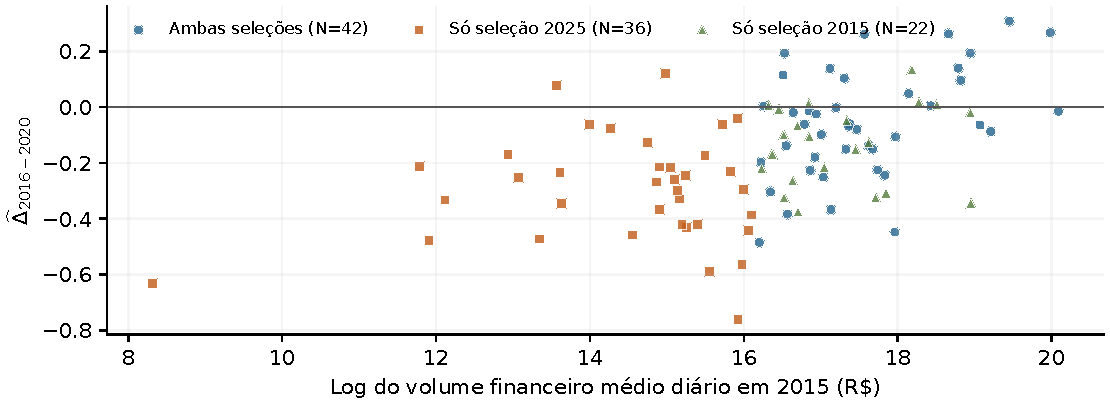
\includegraphics[width=\textwidth]{lab03j_liquidez_inicial.pdf}
\caption{ISINs elegíveis e liquidez inicial. Cada ponto é um ativo sem
peso empresarial; associação de postos não identifica mecanismo causal.}
\label{fig:liquidez}
\end{figure}

Na união de 82 pares, $\rho_S$ entre mudanças de liquidez e de assimetria
é 0,0789, com $p=0,4018$ e Holm 4=0,4276; nos 77 originais, 0,1338 e
Holm 4=0,4276. Não se obtém evidência ajustada de que a melhora da liquidez
acompanhe a mudança de beta. Esse alvo difere da associação com o nível
inicial e não identifica a explicação do deslocamento temporal.

O cruzamento das 83 marcações com tabelas oficiais de capital recuperadas
classifica 41 com fator compatível, 19 como candidatas à grade de um
centavo e 23 sem correspondência. Das 56 marcações em 2016--2025,
37 têm fator compatível e 19 não encontram registro; as demais 27 são
de 2015. Aprovação e quantidade não certificam data ex: nenhuma das 83
recebe homologação econômica integral por esse cruzamento. O suplemento
preserva o inventário e os limites de cobertura das fontes CVM.

\section{Discussão e limitações}
A evidência mais consistente é a distinção entre níveis históricos
agregados, heterogeneidade individual e sensibilidade temporal.
A média da década é negativa na família secundária principal;
identificação individual se concentra em poucos nomes e muda com
observações e especificações. No período recente, estimativas próximas
de zero coexistem com incerteza; não se conclui desaparecimento da assimetria.

A mudança média entre quinquênios recebe evidência na família G4,
mas as exclusões de 2020 não mantêm rejeição na escolha principal H4.
Os sinais continuam positivos. A leitura deve considerar simultaneamente
a redução do contraste, os valores brutos e as famílias distintas.
Não se identifica uma transição estrutural ou um mecanismo causal.
As não rejeições temporais individuais tampouco demonstram constância:
testes de mesmo sinal em todos os anos têm potência muito baixa.

A calibração evita tratar todo intervalo rotulado 95\% como validado.
O desempenho varia por alvo e mecanismo; validade sob leis específicas
não se transfere a outros desenhos ou às máscaras novas. Os diagnósticos
CDF ajudam a caracterizar essa dependência, mas não justificam seleção
de um gerador favorável ou substituição retrospectiva da referência.
Maior precisão Monte Carlo não acrescenta informação empírica ou
resolve incerteza econômica dos retornos.

Seleção por liquidez de 2025, sobrevivência, setores pequenos e versões
revisadas limitam a generalização. Hashes identificam versões, sem
reconstituir informação disponível em cada data. A relação simples
com liquidez se reduz com os controles e não permanece detectada nos
modelos completos após Holm 16. O desenho não distingue risco econômico
de liquidez, negociação infrequente e outros confundidores; tampouco
identifica que a seleção tenha causado a assimetria ou a mudança.
A capitalização aproximada e os casos completos mantêm incerteza de
mensuração e seleção adicional. As análises complementares são
exploratórias, com hipóteses e resultados anteriores conhecidos.

A conciliação econômica integral permanece incompleta, e ICs estatísticos
não incorporam toda a incerteza dos eventos. As sensibilidades de caixa,
lacunas, Light, influência e continuidade permanecem no suplemento.
Retornos excedentes requerem taxa diária autenticada e outro alvo.
A previsão exploratória preservada não prevê beta futuro e não demonstrou
superioridade preditiva nem contribuição própria em IA.

\section{Conclusões}
Nas amostras fixas, a média da assimetria na década é negativa, mas a
identificação individual é frágil e os níveis recentes são inconclusivos.
A detecção da mudança depende da janela e da família; excluir períodos
de 2020 reduz o contraste e perde rejeição na escolha principal.
A seleção por 2015 altera composição e elegibilidade. Liquidez inicial
tem associação simples com assimetria inicial, porém os modelos com
porte, setor e beta tradicional não rejeitam após ajuste. A relação
entre mudanças de liquidez e de assimetria tampouco recebe detecção
ajustada. Esses resultados delimitam uma associação condicionada ao
desenho, sem estabelecer causalidade, equivalência ou estabilidade futura.

A contribuição é uma análise empírica reproduzível da sensibilidade
dos betas condicionais a amostra, mensuração e inferência. Não se
estabelecem assimetria generalizada, ganho econômico ou mecanismo
único. Auditoria econômica e calibração para os desenhos adicionais
permanecem limites explícitos; exposição futura e métodos de
representação/raciocínio requerem investigações próprias.

\section*{Disponibilidade e reprodutibilidade}
Código, protocolos, artigo, suplemento, estimativas e diagnósticos
estão em\url{https://github.com/robsondf/alem-do-beta-gemini};
o histórico de desenvolvimento está em\url{https://github.com/robsondf/alem-do-beta}.
A seleção pública não contém todas as matrizes financeiras necessárias
à reprodução integral, mantidas no Drive. Não foi atribuída nova licença
a materiais de terceiros. O manifesto de proveniência registra hashes
e versões, inclusive o manuscrito anterior de 25 páginas.

As execuções do autor no Colab até as análises de seleção/liquidez
foram conferidas com exports autenticados. As novas regressões,
diagnósticos e três continuidades foram executados localmente e
conferidos por OLS densa independente; a execução do novo notebook
pelo autor é uma etapa distinta, ainda não realizada nesta versão.
Protocolos, entradas públicas, resultados e recibos estão em
\texttt{data/lab03j/} e nas pastas correspondentes. Matrizes diárias
e caches B3 são reutilizados do Drive, sem novas cotações. O experimento
externo de seleção em 2015 foi fornecido no processo de revisão assistido
por IA; seu código foi lido, e a reprodução usa implementação própria,
não execução dos scripts recebidos. Independência de código não equivale
a validação por terceiro humano nem a homologação econômica.

\section*{Uso de inteligência artificial}
ChatGPT/Codex (OpenAI) apoiou planejamento, programação, verificadores,
figuras, busca documental e redação. Responsabilidade pelas escolhas,
referências, interpretação e aprovação final permanece com o autor humano.

\bibliographystyle{sbc}
\bibliography{references_artigo}
\end{document}
